% LaTeX source for ``Think DSP: Digital Signal Processing for Programmers''
% Copyright 2013  Allen B. Downey.

% License: Creative Commons Attribution-NonCommercial 3.0 Unported License.
% http://creativecommons.org/licenses/by-nc/3.0/
%

\documentclass[12pt]{book}
\usepackage[width=5.5in,height=8.5in,
  hmarginratio=3:2,vmarginratio=1:1]{geometry}

% for some of these packages, you might have to install
% texlive-latex-extra (in Ubuntu)

\usepackage[T1]{fontenc}
\usepackage{textcomp}
\usepackage{mathpazo}
\usepackage{url}
\usepackage{graphicx}
\usepackage{subfig}
\usepackage{amsmath}
\usepackage{amsthm}
\usepackage{makeidx}
\usepackage{setspace}
\usepackage{hevea}                           
\usepackage{upquote}
\usepackage{fancyhdr}
\usepackage[bookmarks]{hyperref}

\title{Think DSP}
\author{Allen B. Downey}

\newcommand{\thetitle}{Think DSP: Digital Signal Processing in Python}
\newcommand{\theversion}{0.1}

% these styles get translated in CSS for the HTML version
\newstyle{a:link}{color:black;}
\newstyle{p+p}{margin-top:1em;margin-bottom:1em}
\newstyle{img}{border:0px}

% change the arrows in the HTML version
\setlinkstext
  {\imgsrc[ALT="Previous"]{back.png}}
  {\imgsrc[ALT="Up"]{up.png}}
  {\imgsrc[ALT="Next"]{next.png}} 

\makeindex

\newif\ifplastex
\plastexfalse

\begin{document}

\frontmatter

\ifplastex

\else
\fi

\ifplastex
    \usepackage{localdef}
    \maketitle

\else

\newtheoremstyle{exercise}% name of the style to be used
  {\topsep}% measure of space to leave above the theorem. E.g.: 3pt
  {\topsep}% measure of space to leave below the theorem. E.g.: 3pt
  {}% name of font to use in the body of the theorem
  {0pt}% measure of space to indent
  {\bfseries}% name of head font
  {}% punctuation between head and body
  { }% space after theorem head; " " = normal interword space
  {}% Manually specify head

\theoremstyle{exercise}
\newtheorem{exercise}{Exercise}[chapter]

\input{latexonly}

\begin{latexonly}

\renewcommand{\blankpage}{\thispagestyle{empty} \quad \newpage}

% TITLE PAGES FOR LATEX VERSION

%-half title--------------------------------------------------
\thispagestyle{empty}

\begin{flushright}
\vspace*{2.0in}

\begin{spacing}{3}
{\huge Think DSP}\\
{\Large Digital Signal Processing in Python}
\end{spacing}

\vspace{0.25in}

Version \theversion

\vfill

\end{flushright}

%--verso------------------------------------------------------

\blankpage
\blankpage

%--title page--------------------------------------------------
\pagebreak
\thispagestyle{empty}

\begin{flushright}
\vspace*{2.0in}

\begin{spacing}{3}
{\huge Think DSP}\\
{\Large Digital Signal Processing in Python}
\end{spacing}

\vspace{0.25in}

Version \theversion

\vspace{1in}


{\Large
Allen B. Downey\\
}


\vspace{0.5in}

{\Large Green Tea Press}

{\small Needham, Massachusetts}

\vfill

\end{flushright}


%--copyright--------------------------------------------------
\pagebreak
\thispagestyle{empty}

Copyright \copyright ~2013 Allen B. Downey.


\vspace{0.2in}

\begin{flushleft}
Green Tea Press       \\
9 Washburn Ave \\
Needham MA 02492
\end{flushleft}

Permission is granted to copy, distribute, and/or modify this document
under the terms of the Creative Commons Attribution-NonCommercial 3.0 Unported
License, which is available at \url{http://creativecommons.org/licenses/by-nc/3.0/}.

\vspace{0.2in}

\end{latexonly}


% HTMLONLY

\begin{htmlonly}

% TITLE PAGE FOR HTML VERSION

{\Large \thetitle}

{\large Allen B. Downey}

Version \theversion

\vspace{0.25in}

Copyright 2012 Allen B. Downey

\vspace{0.25in}

Permission is granted to copy, distribute, and/or modify this document
under the terms of the Creative Commons Attribution-NonCommercial 3.0
Unported License, which is available at
\url{http://creativecommons.org/licenses/by-nc/3.0/}.

\setcounter{chapter}{-1}

\end{htmlonly}

\fi
% END OF THE PART WE SKIP FOR PLASTEX

\chapter{Preface}
\label{preface}

The premise of this book (and the other books in the {\it Think X}
series) is that if you know how to program, you can use that skill to
learn other things.  I am writing this book because I think the
conventional approach to digital signal processing is backward: most
books (and the classes that use them) present the material bottom-up,
starting with mathematical abstractions like phasors.

With a programming-based approach, I can go top-down, which means I
can present the most important ideas right away.  By the end of the
first chapter, you can break down a sound into its harmonics, modify
the harmonics, and generate new sounds.

This is a work in progress, so comments are welcome.


Allen B. Downey \\*

Needham MA \\*

Allen B. Downey is a Professor of Computer Science at 
the Franklin W. Olin College of Engineering.



\section*{Contributor List}

If you have a suggestion or correction, please send email to 
{\tt downey@allendowney.com}.  If I make a change based on your
feedback, I will add you to the contributor list
(unless you ask to be omitted).
\index{contributors}

If you include at least part of the sentence the
error appears in, that makes it easy for me to search.  Page and
section numbers are fine, too, but not as easy to work with.
Thanks!

\small

\begin{itemize}

\item 

% ENDCONTRIB

\end{itemize}

\normalsize

\clearemptydoublepage

% TABLE OF CONTENTS
\begin{latexonly}

\tableofcontents

\clearemptydoublepage

\end{latexonly}

% START THE BOOK
\mainmatter


\chapter{Sounds and signals}
\label{sounds}

A {\bf signal} is a representation of a quantity that varies in time,
or space, or both.  That definition is pretty abstract, so let's start
with a concrete example, sound.  Sound is variation in air pressure.
A sound signal represents variations in air pressure over time.

A microphone is a device that measures these variations and generates
an electronic signal that represents sound.  A speaker is a device
that takes an electrical signal and produces sound.
Microphones and speakers are called {\bf transducers} because they
transduce, or convert, signals from one form to another.

This book is about signal processing, which includes processes for
synthesizing, transforming, and analyzing signals.  It focuses on
sound signals, but the same methods apply to other signals, like
electronic signals and mechanical vibration.

They also apply to signals that vary in space rather than time, like
elevation along a hiking trail.

And they apply to signals in more than one dimension, like an
image, which you can think of as a signal that varies in two-dimensional
space (or three).  Or a movie, which is a signal that varies
in two-dimensional space {\it and} time.

But we'll start with simple one-dimensional sound.


\section{Periodic signals}

\begin{figure}
% violin.py
\centerline{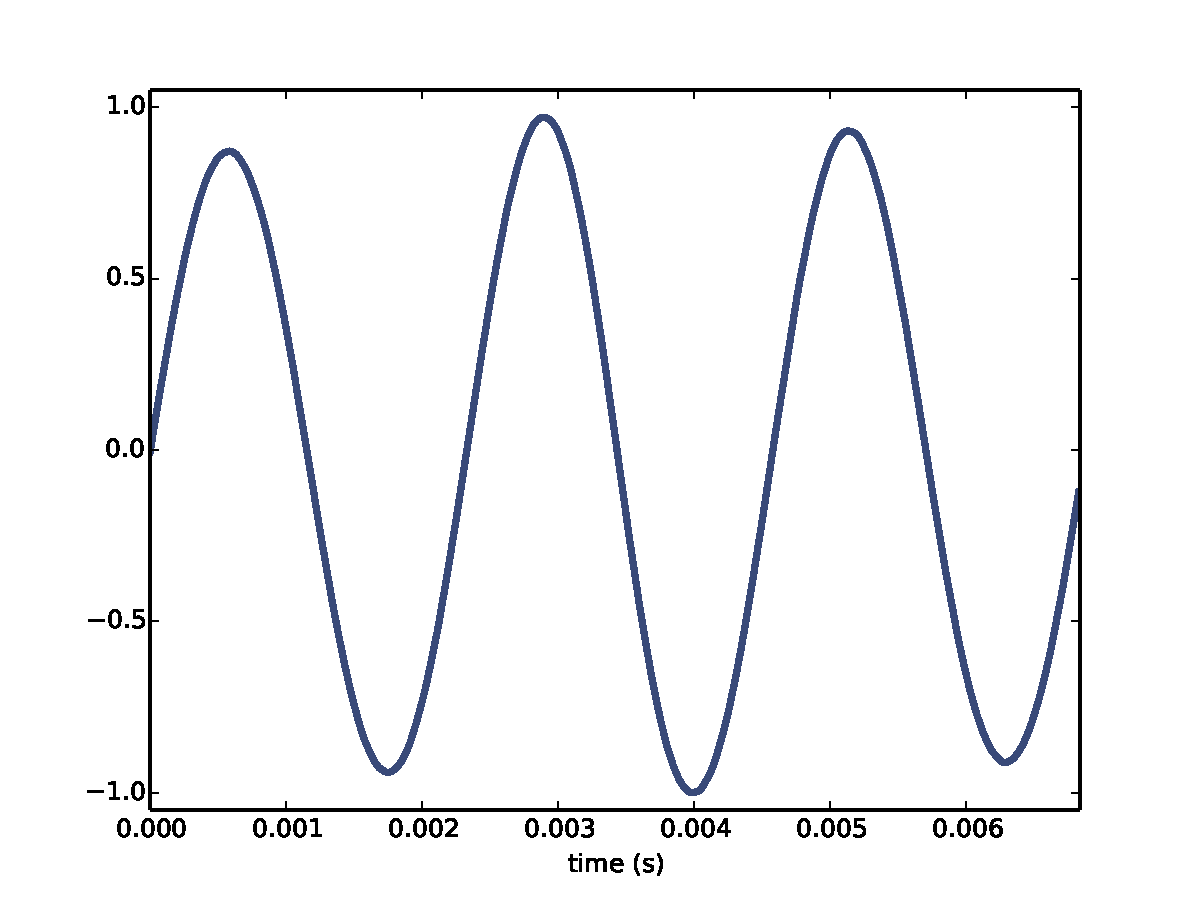
\includegraphics[height=2.5in]{figs/tuning1.pdf}}
\caption{Short sample from a recording of a tuning fork.}
\label{fig.tuning1}
\end{figure}


We will also start with {\bf periodic signals}, which are signals
that repeat themselves after some period.  For example, if you
strike a tuning fork, it vibrates and generates sound.  If you
record that sound and plot the transduced signal, it looks like
Figure~\ref{fig.tuning1}.\footnote{I got this recording from
\url{http://www.freesound.org/people/zippi1/sounds/18871/}.}

This signal is a sinusoid, which means it has the same shape as
the trigonometric sine function. 

You can see that this signal is periodic.  I chose the duration
to show three full periods, also known as {\bf cycles}.
The duration of each cycle is
about 2.3 ms.

The {\bf frequency} of a signal is the number of cycles
per second, which is the inverse of the period.
The units of frequency are cycles per second, or {\bf Hertz},
abbreviated ``Hz''.

The frequency of this signal is about 439 Hz, slightly lower than 440
Hz, which is the standard tuning pitch for orchestral music.  The
musical name of this note is A, or more specifically, A4.  If you are
not familiar with ``scientific pitch notation'', the suffix indicates
which octave the note is in.  A4 is the A above middle C.  A5 is one
octave higher.  See
\url{http://en.wikipedia.org/wiki/Scientific_pitch_notation}.

\begin{figure}
% violin.py
\centerline{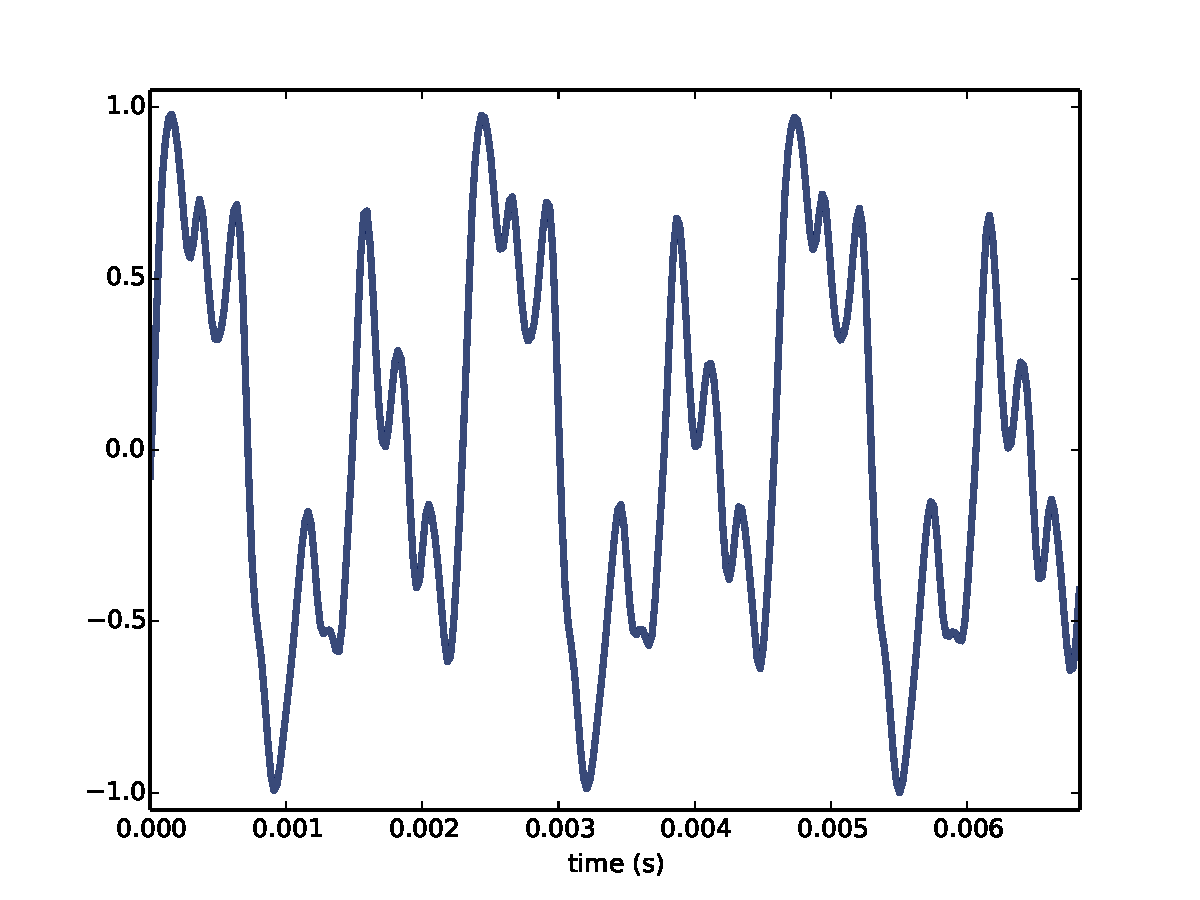
\includegraphics[height=2.5in]{figs/violin1.pdf}}
\caption{Short sample from a recording of a violin.}
\label{fig.violin1}
\end{figure}

A tuning fork generates a sinusoid because the vibration of the tines
is a form of simple harmonic motion.  Most musical instruments
produce periodic signals, but the shape of these signals is not
sinusoidal.  For example, Figure~\ref{fig.violin1} shows a sample
from a recording of a violin playing
Boccherini's String Quintet No. 5 in E, 3rd
movement.\footnote{The recording is from
  \url{http://www.freesound.org/people/jcveliz/sounds/92002/}.
I identified the piece using \url{http://www.musipedia.org}.}

Again we can see that the signal is periodic, but the shape of the
signal is much more complex.  The shape of a periodic signal is called
the {\bf waveform}.  Most musical instruments produce waveforms more
complex than a sinusoid.  The shape of the waveform determines the
musical {\bf timbre}, which is our perception of the tone quality of the
sound.  People usually perceive complex waveforms as rich, warm and
more interesting than sinusoids.


\section{Spectral decomposition}

\begin{figure}
% violin.py
\centerline{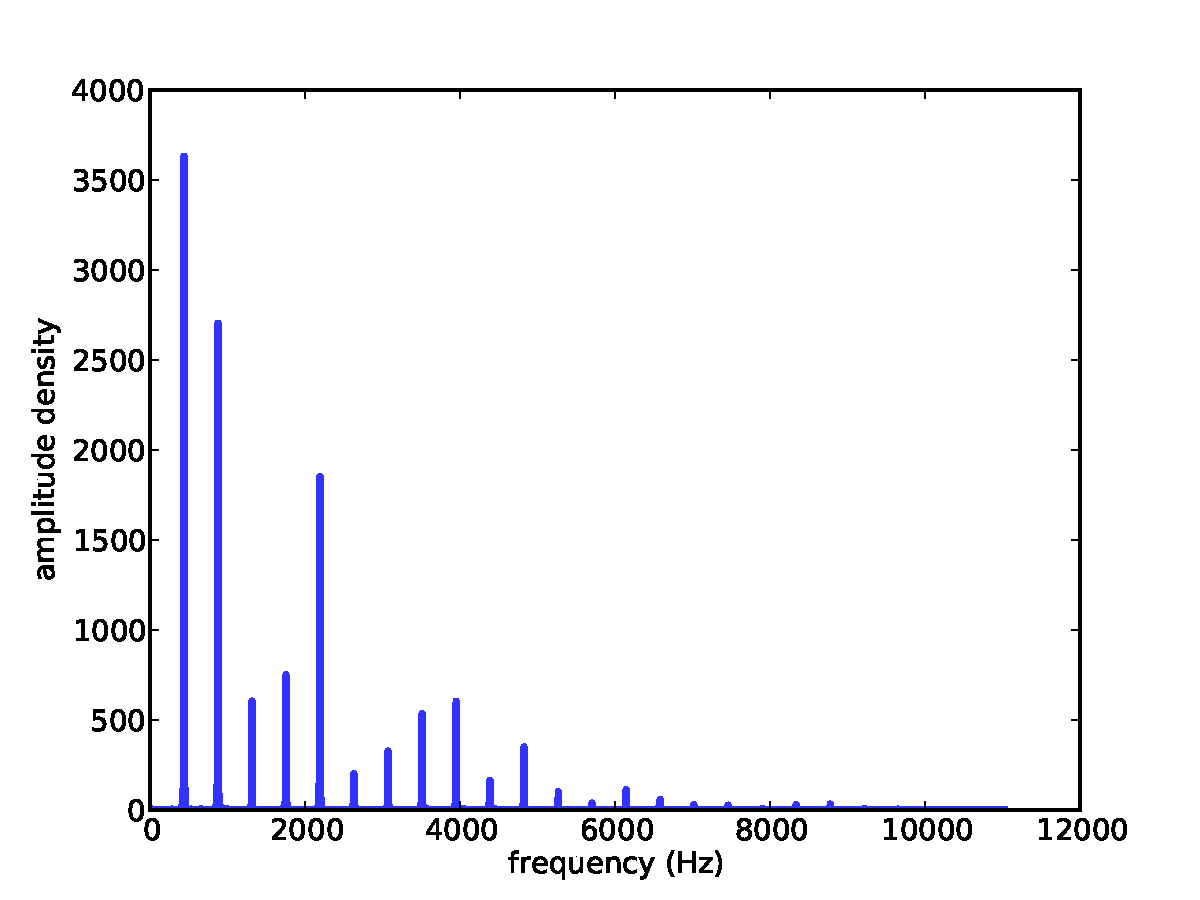
\includegraphics[height=2.5in]{figs/violin2.pdf}}
\caption{Spectrum of the violin sample.}
\label{fig.violin2}
\end{figure}

The most important idea in this book is {\bf spectral decomposition},
which is the idea that a complex signal can be expressed as the sum of
simpler signals with different frequencies.

And the most important algorithm in this book is the {\bf discrete
  Fourier transform}, or {\bf DFT}, which takes a signal (a quantity
varying in time) and produces its {\bf spectrum}, which is the set of
sinusoids that add up to produce the signal.

For example, Figure~\ref{fig.violin2} shows the spectrum of the violin
sample in Figure~\ref{fig.violin1}.  The x-axis is the range of
frequencies that make up the signal.  The y-axis shows the strength of
each frequency component.  The units of the y-axis are complicated;
I will explain more later.

The lowest frequency component is called the {\bf fundamental
  frequency}.  The fundamental frequency of this signal is near 440 Hz
(actually a little lower, or ``flat'').

In this signal the fundamental frequency has the largest amplitude,
so it is also the {\bf dominant frequency}.

Normally the perceived pitch of a sound is determined by the
fundamental frequency, even if it is not dominant. 

The other spikes in the spectrum are at frequencies 880, 1320, 1760, and
2200, which are integer multiples of the fundamental.
These components are called {\bf harmonics} because they are
musically harmonious with the fundamental:

\begin{itemize}

\item 880 is the frequency of
A5, one octave higher than the fundamental.  

\item 1320 is approximately E6, which is a major fifth above A5.

\item 1760 is A6, two octaves above the fundamental. 

\item 2200 is approximately C$\sharp$7, which is a major third
above A6.

\end{itemize}

In other words, these harmonics make up the notes of an A major
chord, although not all in the same octave.  Some of them are only
approximate because the notes that make up Western music have been
adjusted for {\bf equal temperament} (see
 \url{http://en.wikipedia.org/wiki/Equal_temperament}).

Given the harmonics and their amplitudes, you can reconstruct the
signal (at least approximately) by adding up sinusoids.  Or, to
reconstruct the signal exactly, you can use the inverse DFT.  
Next we'll see how.


\section{Signals}

I wrote a Python module called {\tt thinkdsp} that contains
classes and function for working with signals and spectrums.
\footnote{In Latin the plural of ``spectrum'' is ``spectra'', but I
prefer to use standard English plurals.}  You can download
it from \url{http://think-dsp.com/thinkdsp.py}.

To represent signals, {\tt thinkdsp} provides a class named
{\tt Signal}, which is the parent class for several signal types,
including {\tt Sinusoid}, which represents both sine and cosine
signals.

{\tt thinkdsp} provides functions to create sine and cosine signals:

\begin{verbatim}
    cos_sig = thinkdsp.CosSignal(freq=440, amp=1.0, offset=0)
    sin_sig = thinkdsp.SinSignal(freq=880, amp=0.5, offset=0)
\end{verbatim}

{\tt freq} is frequency in Hz.  {\tt amp} is amplitude in arbitrary
units.  {\tt offset} is a {\tt phase offset} in radians.

The phase offset determines where in the period the signal starts
(that is, when {\tt t=0}).  For example, a cosine signal with {\tt
  offset=0} starts at $\cos 0$, which is 1.  With {\tt offset=pi/2} it
starts at $\cos \pi/2$, which is 0.
A sine signal with
{\tt offset=0} also starts at 0.  In fact,
a cosine signal with {\tt offset=pi/2} is identical to a sine
signal with {\tt offset=0}.

Signals have an \verb"__add__" method, so you can use the {\tt +}
operator to add them:

\begin{verbatim}
    mix = sin_sig + cos_sig
\end{verbatim}

The result is a {\tt SumSignal}, which represents the sum of two
or more signals.

A Signal is basically a Python representation of a mathematical
function.  Most signals are defined for all values of {\tt t},
from negative infinity to infinity.

But you can't do much with a
Signal until you evaluate it.
In this context, ``evaluate'' means taking a sequence of {\tt ts}
and computing the corresponding values of the signal, which I
call {\tt ys}.  I encapsulate {\tt ts} and {\tt ys} in an
object called a Wave.

A Wave represents a signal evaluated at a sequence of points in
time.  Each point in time is called a {\bf frame} (a term borrowed
from movies and video).

{\tt Signal} provides \verb"make_wave", which returns a new
Wave object:

\begin{verbatim}
    wave = mix.make_wave(duration=0.5, start=0, framerate=11025)
\end{verbatim}

{\tt duration} is the length of the Wave in seconds.  {\tt start} is
the start time, also in seconds.  {\tt framerate} is the (integer)
number of frames per second.

This example evaluates the signal from {\tt t=0} to {\tt t=0.5} at
5513 equally-spaced frames (because 5513 is half of 11025).
The time between frames, or {\bf timestep}, is {\tt 1/11025} seconds, or
91 $\mu$s.

{\tt Wave} provides a {\tt plot} method that uses {\tt pyplot}.
You can plot the wave like this:

\begin{verbatim}
    wave.plot()
    pyplot.show()
\end{verbatim}

\begin{figure}
% example1.py
\centerline{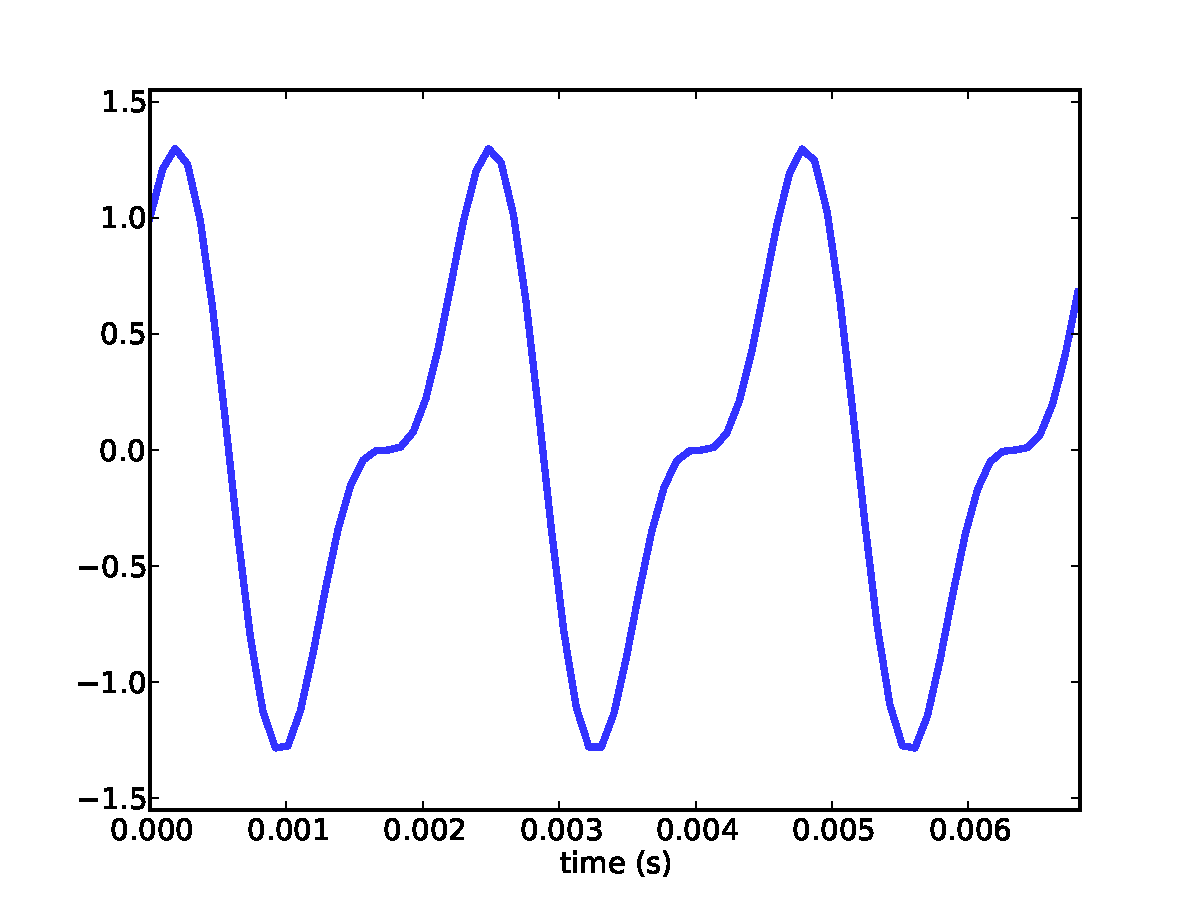
\includegraphics[height=2.5in]{figs/example1.pdf}}
\caption{Short sample from a mixture of two sinusoid signals.}
\label{fig.example1}
\end{figure}

At {\tt freq=440} there are 220 periods in 0.5 seconds,
so the plot just looks like a solid block.  To zoom in on a small
number of periods, we can use {\tt sample}, which copies a segment
of a Wave and returns a new wave:

\begin{verbatim}
    period = mix.period
    sample = wave.sample(start=0, duration=period*3)
\end{verbatim}

{\tt start} and {\tt duration} are in seconds.  This example copies
the first three periods from {\tt mix}.  If we plot the sample, it
looks like Figure~\ref{fig.example1}.  This signal contains two
frequency components, so it is more complex than the signal from the
tuning fork, but less complex than the violin.


\section{Reading and writing Waves}

{\tt thinkdsp} provides \verb"read_wave", which reads a WAV
file and returns a Wave:

\begin{verbatim}
    violin_wave = thinkdsp.read_wave('violin1.wav')
\end{verbatim}

And {\tt Wave} provides {\tt write}, which writes a WAV file:

\begin{verbatim}
    wave.write(filename='example1.wav')
\end{verbatim}

You can listen to Wave with any media player that plays WAV
files.  On UNIX systems, I use {\tt aplay}, which is simple, robust,
and included in many Linux distributions.  For Windows you might like
MicroWav, available from
\url{http://bellsouthpwp2.net/b/o/bobad/microwav.htm}.

{\tt thinkdsp} also provides \verb"play_wave", which runs
the media player as a subprocess:

\begin{verbatim}
    thinkdsp.play_wave(filename='example1.wav', player='aplay')
\end{verbatim}

It uses {\tt aplay} by default, but you can provide another player.


\section{Spectrums}

{\tt Wave} provides \verb"make_spectrum", which returns a
{\tt Spectrum}:

\begin{verbatim}
    spectrum = wave.make_spectrum()
\end{verbatim}

{\tt Spectrum} provides {\tt plot}:

\begin{verbatim}
    spectrum.plot()
    thinkplot.show()
\end{verbatim}

{\tt thinkplot} is a module I wrote to provide wrappers around some of
the functions in {\tt matplotlib}.  You can download it from
\url{http://think-dsp.com/thinkplot.py}.  It is also included in the
Git repository for this book (see Section~\ref{code}).

{\tt Spectrum} also provides three methods that modify the spectrum:

\begin{itemize}

\item \verb"low_pass" applies a low-pass filter, which means that
  components above a given cutoff frequency are attenuated (that is,
  reduced in magnitude) by a factor.

\item \verb"high_pass" applies a high-pass filter, which means that
  it attenuates components below the cutoff.

\item \verb"band_stop" attenuates components in a the band of
frequencies between two cutoffs.

\end{itemize}

This example attenuates all frequencies above 600 by 99\%:

\begin{verbatim}
   spectrum.low_pass(cutoff=600, factor=0.01)
\end{verbatim}

Finally, you can convert a Spectrum back to a Wave:

\begin{verbatim}
    wave = spectrum.make_wave()
\end{verbatim}

At this point you know how to use many of the classes and functions in
{\tt thinkdsp}, and you are ready to do the exercises at the end of
the chapter.  In Chapter~\ref{implementation} I will explain more
about how these classes are implemented.



\section{Exercises}

\begin{exercise}
Read the thinkdsp documentation.
\end{exercise}

\begin{exercise}
Fork and clone the repo.
\end{exercise}

\begin{exercise}
Run example1.py and listen.
\end{exercise}

\begin{exercise}
Run violin.py and listen.
\end{exercise}

\begin{exercise}
Create exercise1.py and copy example1.py

Record a WAV file, or download from ...

Use an audio editor to examine the wave

Find a section where the wave is periodic and plot a few periods.

Compute and plot the spectrum.
\end{exercise}

\begin{exercise}
Extract a 0.5-2 second sample with constant frequency.

Compute the spectrum.

Remove some of the harmonics, invert the transform and play the wave.
\end{exercise}

\begin{exercise}
Synthesize a wave by creating a spectrum with arbitrary harmonics,
inverting it, and listening.  What happens as you add frequency
components that are not multiples of the fundamental?
\end{exercise}




\chapter{Fast Fourier Transform}
\label{implementation}

\section{Implementing Signals and Spectrums}

If you have done the exercises, you know how to use the
classes and methods in {\tt thinkdsp}.  Now we'll see how
some of it works.

We'll start with {\tt CosSignal} and {SinSignal}:

\begin{verbatim}
def CosSignal(freq=440, amp=1.0, offset=0):
    return Sinusoid(freq, amp, offset, func=numpy.cos)

def SinSignal(freq=440, amp=1.0, offset=0):
    return Sinusoid(freq, amp, offset, func=numpy.sin)
\end{verbatim}

These functions are just wrappers for {\tt Sinusoid}, which
is a kind of Signal:

\begin{verbatim}
class Sinusoid(Signal):
    
    def __init__(self, freq=440, amp=1.0, offset=0, func=numpy.sin):
        Signal.__init__(self)
        self.freq = freq
        self.amp = amp
        self.offset = offset
        self.func = func
\end{verbatim}

The parameters of \verb"__init__" are:

\begin{itemize}

\item {\tt freq}: frequency in cycles per second, or Hz.

\item {\tt amp}: amplitude.  The units of amplitude are arbitrary,
usually chosen so 1.0 corresponds to the maximum output of a
microphone or maximum input of a speaker.

\item {\tt offset}: where in its period the signal starts, at $t=0$.
In units of radians, for reasons I explain below.

\item {\tt func}: a Python function or function-like object used
to evaluate the signal at a particular point in time.  It is
usually either {\tt sin} or {\tt cos}, yielding a sine or
cosine signal.

\end{itemize}

Like many \verb"__init__" methods, this one just tucks the
parameters away for future use.

The parent class of {\tt Sinusoid}, {\tt Signal}, provides \verb"make_wave":

\begin{verbatim}
    def make_wave(self, duration=1, start=0, framerate=11025):
        """Makes a Wave object.

        duration: float seconds
        start: float seconds
        framerate: int frames per second

        returns: Wave
        """
        dt = 1.0 / framerate
        ts = numpy.arange(start, duration, dt)
        ys = self.evaluate(ts)
        return Wave(ys, framerate)
\end{verbatim}

\verb"make_wave" invokes {\tt evaluate}, which has to be provided
by the child class of {\tt Signal}, in this case {\tt Sinusoid}.

{\tt evaluate} takes an array of time values and returns an array of
corresponding quantities:

\begin{verbatim}
    def evaluate(self, ts):
        phases = PI2 * self.freq * ts + self.offset
        ys = self.amp * self.func(phases)
        return ys
\end{verbatim}

{\tt ts} and {\tt ys} are NumPy arrays.  I use NumPy and SciPy
throughout the book.  If you are familiar with these libraries,
that's great, but I will also explain as we go along.

Let's unwind this function one step at time:

\begin{enumerate}

\item {\tt self.freq} is frequency in cycles per second, and
each element of {\tt ts} a time in seconds, so their product is
the number of cycles since {\tt t=0}.

\item {\tt PI2} is a constant that stores $2 \pi$.  Multiplying
by {\tt PI2} converts from cycles to {\bf phase}.  You can
think of phase as ``cycles since {\tt t=0}'' except that the number
of cycles is in units of radians, so each cycle is $2 \pi$ radians.

\item {\tt self.offset} is the phase, in radians, at {\tt t=0}.  It has
the effect of shifting the signal left or right in time.

\item If {\tt self.func} is {\tt sin} or {\tt cos}, the result is
a value between $-1$ and $+1$.

\item Multiplying by {\tt self.amp} yields a signal that ranges
from {\tt -self.amp} to {\tt +self.amp}.

\end{enumerate}

In math notation, {\tt evaluate} is written like this:

\[ A \cos (2 \pi f t + \phi) \]

where $A$ is amplitude, $f$ is frequency, $t$ is time, and $\phi$
is the phase offset.  It may seem like I wrote a lot of code
to evaluate one simple function, but as we will see, this code
provides a framework for dealing with all kinds of signals, not
just sinusoids.


\section{Computing the spectrum}

Given a Signal, we can compute a Wave.  Given a Wave, we can compute
a Spectrum.  {\tt Wave} provides \verb"make_spectrum", which returns
a new {\tt Spectrum} object.

\begin{verbatim}
    def make_spectrum(self):
        hs = numpy.fft.rfft(self.ys)
        return Spectrum(hs, self.framerate)
\end{verbatim}

\verb"make_spectrum" uses {\tt rfft}, which computes
the discrete Fourier transform using an algorithm called
{\bf Fast Fourier Transform} or FFT.

The result of the FFT is a sequence of complex numbers, {\tt hs},
which is stored in a Spectrum.  There are two ways to think about
complex numbers:

\begin{itemize}

\item A complex number is the sum of a real part and an imaginary
part, often written $x + iy$, where $i$ is the imaginary unit, $\sqrt{1}$.
You can think of $x$ and $y$ as Cartesian coordinates.

\item A complex number is also the product of a magnitude
and a complex exponential, $r e^{i \phi}$, where $r$ is the
{\bf magnitude} and $\phi$ is the
{\bf angle} in radians, also called the ``argument.''   You
can think of $r$ and $\phi$ as polar coordinates.

\end{itemize}

Each element of {\tt hs} corresponds to a
frequency component.  The magnitude of each element is proportional
to the amplitude of the corresponding component.
The angle of each element is the phase offset (relative to a cosine
signal).

{\tt NumPy} provides {\tt absolute}, which computes
the magnitude of a complex number, also called the ``absolute value,''
and {\tt angle}, which computes the angle.

Here is the definition of {\tt Spectrum}:

\begin{verbatim}
class Spectrum(object):

    def __init__(self, hs, framerate):
        self.hs = hs
        self.framerate = framerate

        n = len(hs)
        f_max = framerate / 2.0
        self.fs = numpy.linspace(0, f_max, n)

        self.amps = numpy.absolute(self.hs)
\end{verbatim}

Again, {\tt hs} is the result of the FFT and {\tt framerate}
is the number of frames per second.

The elements of {\tt hs} correspond to a range of frequencies, {\tt
  fs}, equally spaced from 0 to the maximum frequency, \verb"f_max".
The maximum frequency is {\tt framerate/2}, for reasons I'll explain
later.

I'm sorry if these promises to ``explain later'' are irritating, but
I think it is a good idea to practice using these technique first, and
then I'll explain how they work.

Finally, {\tt amps} contains the magnitude of {\tt hs}, which
is proportional to the amplitude of the components.

{\tt Spectrum} provides {\tt plot}, which plots the magnitude for each
frequency:

\begin{verbatim}
    def plot(self, low=0, high=None):
        thinkplot.Plot(self.fs[low:high], self.amps[low:high])
\end{verbatim}

{\tt low} and {\tt high} specify the slice of the Spectrum that
should be plotted.


\section{}


\begin{verbatim}
\end{verbatim}


\begin{verbatim}
\end{verbatim}


\begin{verbatim}
\end{verbatim}


\begin{verbatim}
\end{verbatim}


\begin{verbatim}
\end{verbatim}


\begin{verbatim}
\end{verbatim}


\begin{verbatim}
\end{verbatim}


\begin{verbatim}
\end{verbatim}


\begin{verbatim}
\end{verbatim}


\begin{verbatim}
\end{verbatim}


\begin{verbatim}
\end{verbatim}


\begin{verbatim}
\end{verbatim}


\begin{verbatim}
\end{verbatim}


\begin{verbatim}
\end{verbatim}


\begin{verbatim}
\end{verbatim}



\end{document}
